\documentclass[conference]{IEEEtran}
\IEEEoverridecommandlockouts
% The preceding line is only needed to identify funding in the first footnote. If that is unneeded, please comment it out.
%Template version as of 6/27/2024
\usepackage{cite}
\usepackage{amsmath,amssymb,amsfonts}
\usepackage{algorithmic}
\usepackage{graphicx}
\usepackage{textcomp}
\usepackage{xcolor}
\usepackage{float}
\usepackage{hyperref}
\usepackage{subcaption}
\bibliographystyle{ieeetr}
\renewcommand{\abstractname}{Resumo}
\def\BibTeX{{\rm B\kern-.05em{\sc i\kern-.025em b}\kern-.08em
    T\kern-.1667em\lower.7ex\hbox{E}\kern-.125emX}}
\begin{document}

\title{Relatório Trabalho 1 - Introdução ao Processamento de Imagens
}

\author{\IEEEauthorblockN{Erick Rodrigues Fraga}
\IEEEauthorblockA{\textit{Dep. Ciência da Computação} \\
\textit{Universidade de Brasília}\\
Brasília, Brasil \\
190086815@aluno.unb.br}
}

\maketitle

\begin{abstract}
O primeiro trabalho da matéria de Introdução ao Processamento de Imagens tem como objetivo testar o entendimento dos conceitos apresentados em aula, como a representação de uma imagem pelo computador, 
como amostrar um sinal contínuo de forma discreta, filtros de suavização e aguçamento de imagens em diferentes domínios. Neste trabalho são implementadas funções que efetuam a manipulação e a filtragem de imagens utilizando as bilbiotecas Numpy e OpenCV.
\end{abstract}

\begin{IEEEkeywords}
Convolução, OpenCV, Filtro ideal no domínio da frequência, Filtro Laplaciano, Filtro Gaussiano
\end{IEEEkeywords}

\section{Introdução}
Neste relatório são apresentados de forma resumida os conceitos necessários para solução
das questões pedidas em três partes no trabalho, sendo elas:
\begin{enumerate}
    \item Manipulação do tamanho de imagens.
    \item Aguçamento de imagem utilizando filtros Laplacianos e filtros Gaussianos.
    \item Remoção ou atenuação do efeito Moiré em uma imagem.
\end{enumerate} 
Todas as fórmulas e conceitos aqui aplicados são motivados pelo livro \textit{Digital Image Processing}\cite{gonzalez_digital_2017}, com os mesmos sendo apresentados em aula pelo professor \textit{Bruno Macchiavello}.

Na primeira parte do trabalho, trabalhamos exclusivamente com a imagem no domínio espacial. Aqui, acessamos diretamente os valores de cada píxel da imagem e as alterações que ocorrem são efetuadas diretamente no endereço acessado da matriz.
Neste ponto, é pedido que sejam implementadas funções que transformam o tamanho final da imagem, sendo respectivamente:
\begin{itemize}
    \item Retirar metade das linhas
    \item Retirar metade das colunas
    \item Retirar metade das linhas e das colunas
    \item Dobrar a quantidade de linhas
    \item Dobrar a quantidade de colunas
    \item Dobrar a quantidade de linhas e colunas
\end{itemize}
As implementações das funções devem lidar tanto com entradas monocromáticas quanto coloridas, com a implementação para as imagens coloridas sendo em cada um dos canais de cor da imagem colorida.

Já na segunda parte do trabalho, é necessário trabalhar com a imagem tanto no domínio espacial quanto no domínio da frequência. Utilizando os conceitos apresentados nas aulas 8\cite{macchiavello_dominio_nodate} e 9\cite{macchiavello_dominio_2026}, 
utilizamos a \textit{Transformada de Fourier} para efetuarmos a convolução em uma imagem no domínio da frequência, comparando a aplicação de filtros em cada domínio.

A terceira parte do trabalho, de lidar com o efeito Moiré no domínio da frequência não foi executada neste trabalho.
Por fim, são discutidos os resultados obtidos e as escolhas para as formas de resolução de cada um dos problemas propostos.

\section{Metodologia}
\subsection{Manipulação de Tamanho}
Utilizando uma foto do rosto, nesta parte do projeto é necessário manipular o tamanho de uma imagem tanto reduzindo quanto aumentando o seu tamanho.
Na parte de redução, é necessário a remoção alternada de linhas, colunas e então a aplicação de ambos em uma mesma imagem.
Para a representação digital de uma imagem, temos que a mesma é uma matriz em memória, como apresentado na fórmula:
\begin{equation}
    \label{math:matrix_full}
    I \in \mathbb{Z}^{M \times N}, \quad
    I = \begin{smallmatrix}
    I(1,1) & I(1,2) & \cdots & I(1,N) \\
    I(2,1) & I(2,2) & \cdots & I(2,N) \\
    \vdots  & \vdots  & \ddots & \vdots  \\
    I(M,1) & I(M,2) & \cdots & I(M,N)
    \end{smallmatrix}
\end{equation}
Dessa forma, podemos controlar o tamanho de uma imagem apenas ao diminuir ou aumentar o tamanho da matriz de representação.
\subsubsection{Redução de Tamanho}
Para diminuir o número de linhas e colunas de forma intercalada em uma imagem, podemos criar novas matrizes que guardam apenas os valores dos píxeis em índices pares, das formas
\begin{align}
    \label{math:matrix_evens}
    I_{rrows} \in \mathbb{Z}^{M \times N}, N \in 2\mathbb{Z}\\
    I_{rcols} \in \mathbb{Z}^{M \times N}, M \in 2\mathbb{Z}
\end{align}
\begin{figure}[h!t]
    \label{fig:comparação_redução}
    \centering
    \begin{subfigure}[ht]{0.16\textwidth}
        \centering
        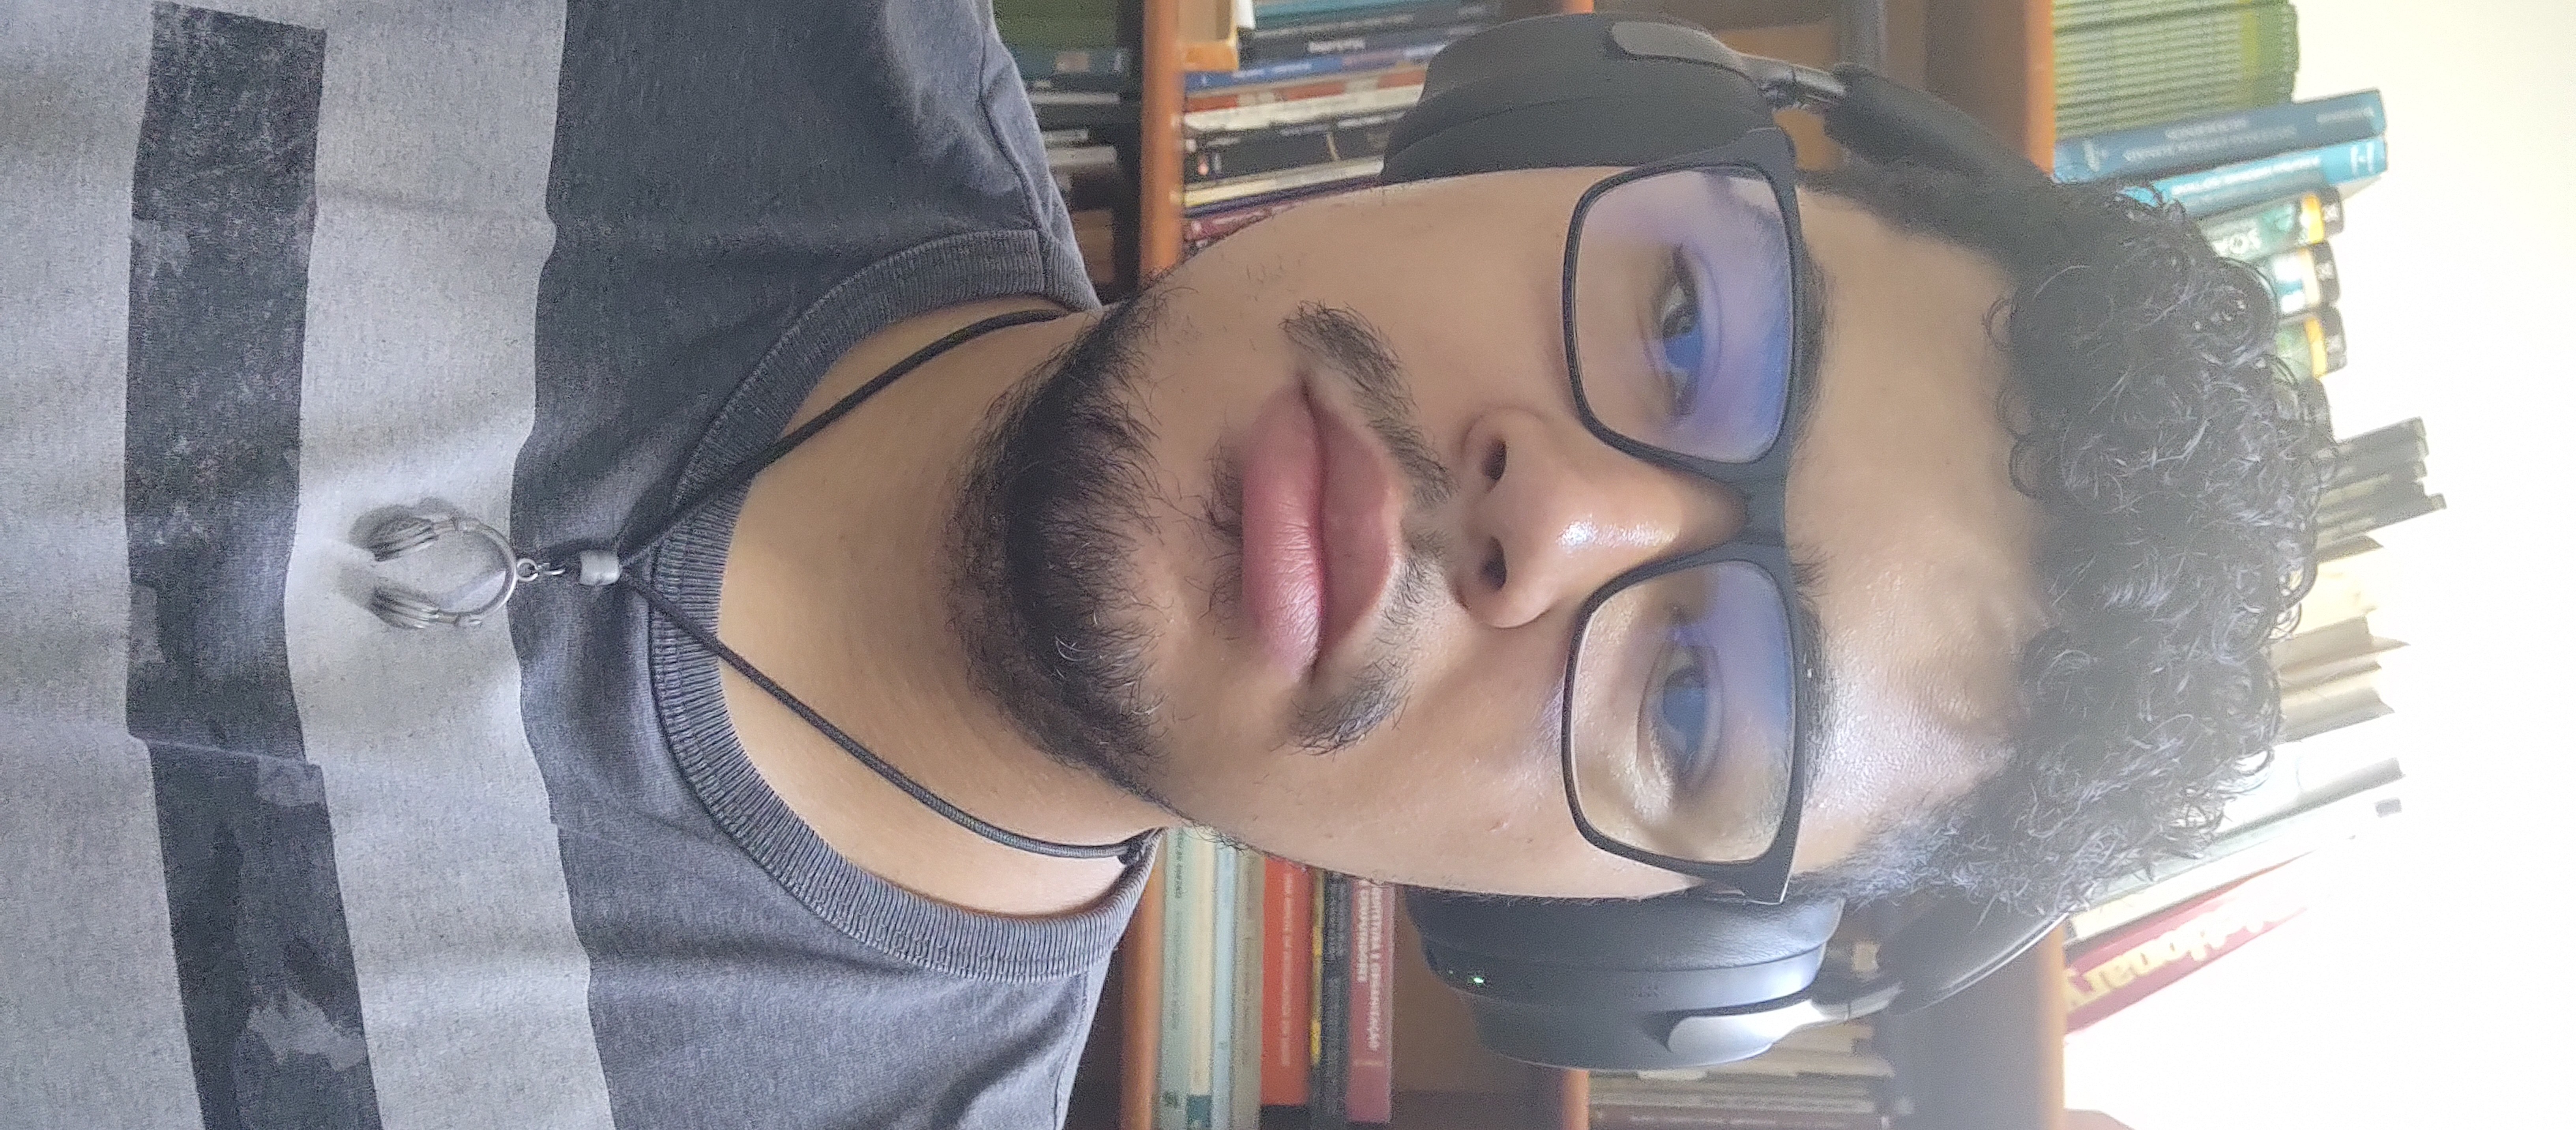
\includegraphics[scale=0.02, angle=90]{img/rosto.jpg}
        \caption{\label{fig:Rosto_Full}Foto com tamanho original.}
    \end{subfigure}
    \quad
    \begin{subfigure}[ht]{0.16\textwidth}
        \centering
        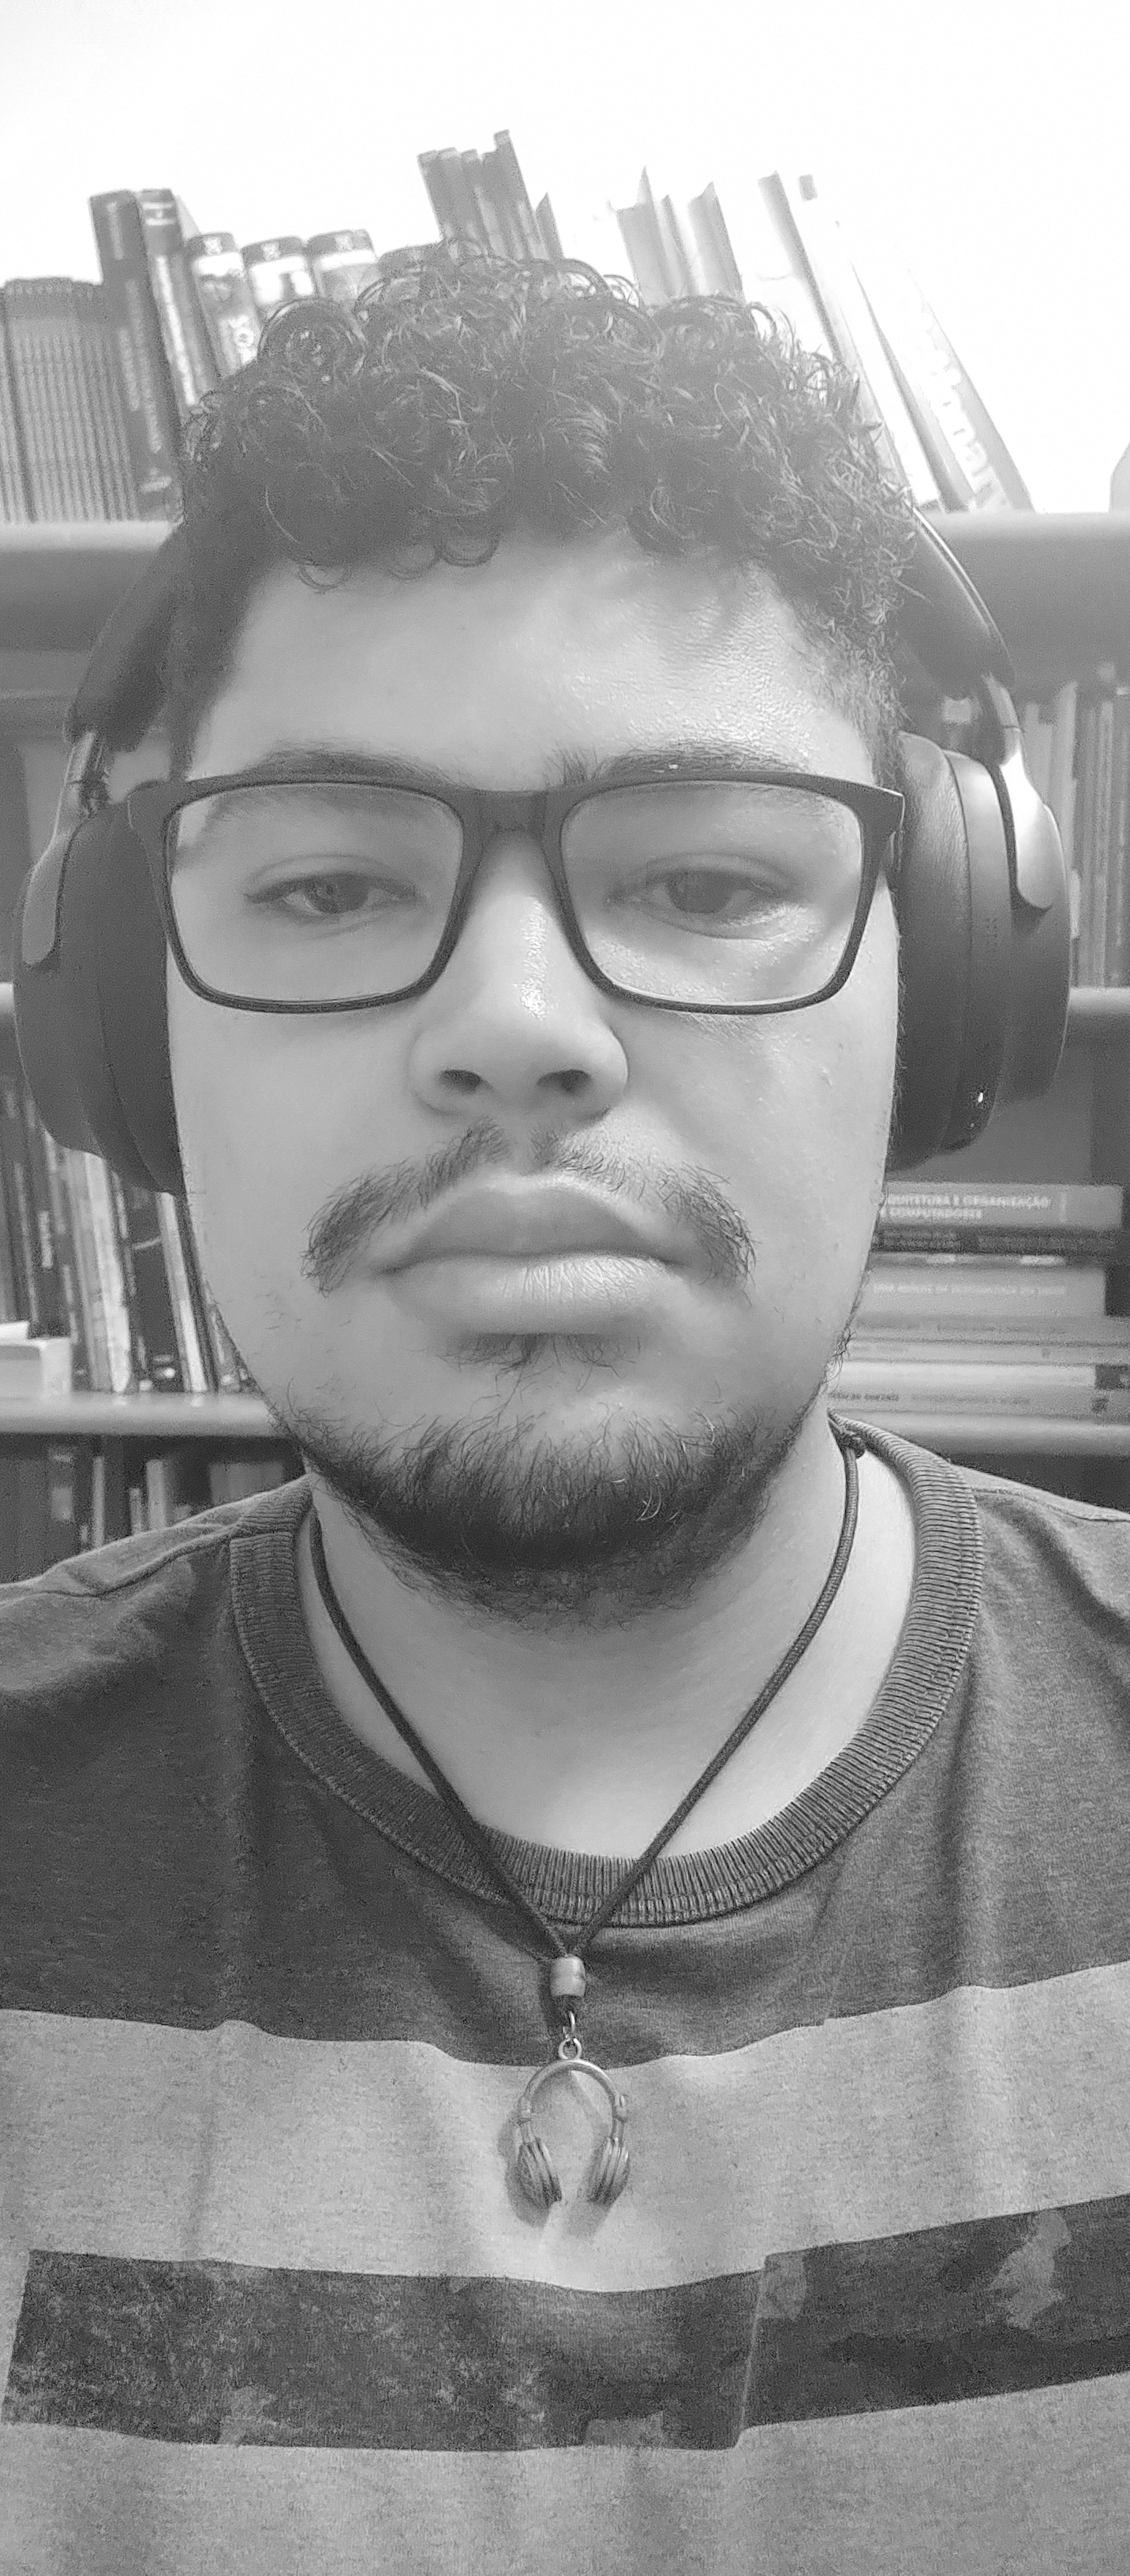
\includegraphics[scale=0.04]{img/saida_redux.png}
        \caption{\label{fig:Rosto_grayscale}Foto grayscale com 1/4 do tamanho original.}
    \end{subfigure}
    \quad
    \begin{subfigure}[ht]{0.16\textwidth}
        \centering
        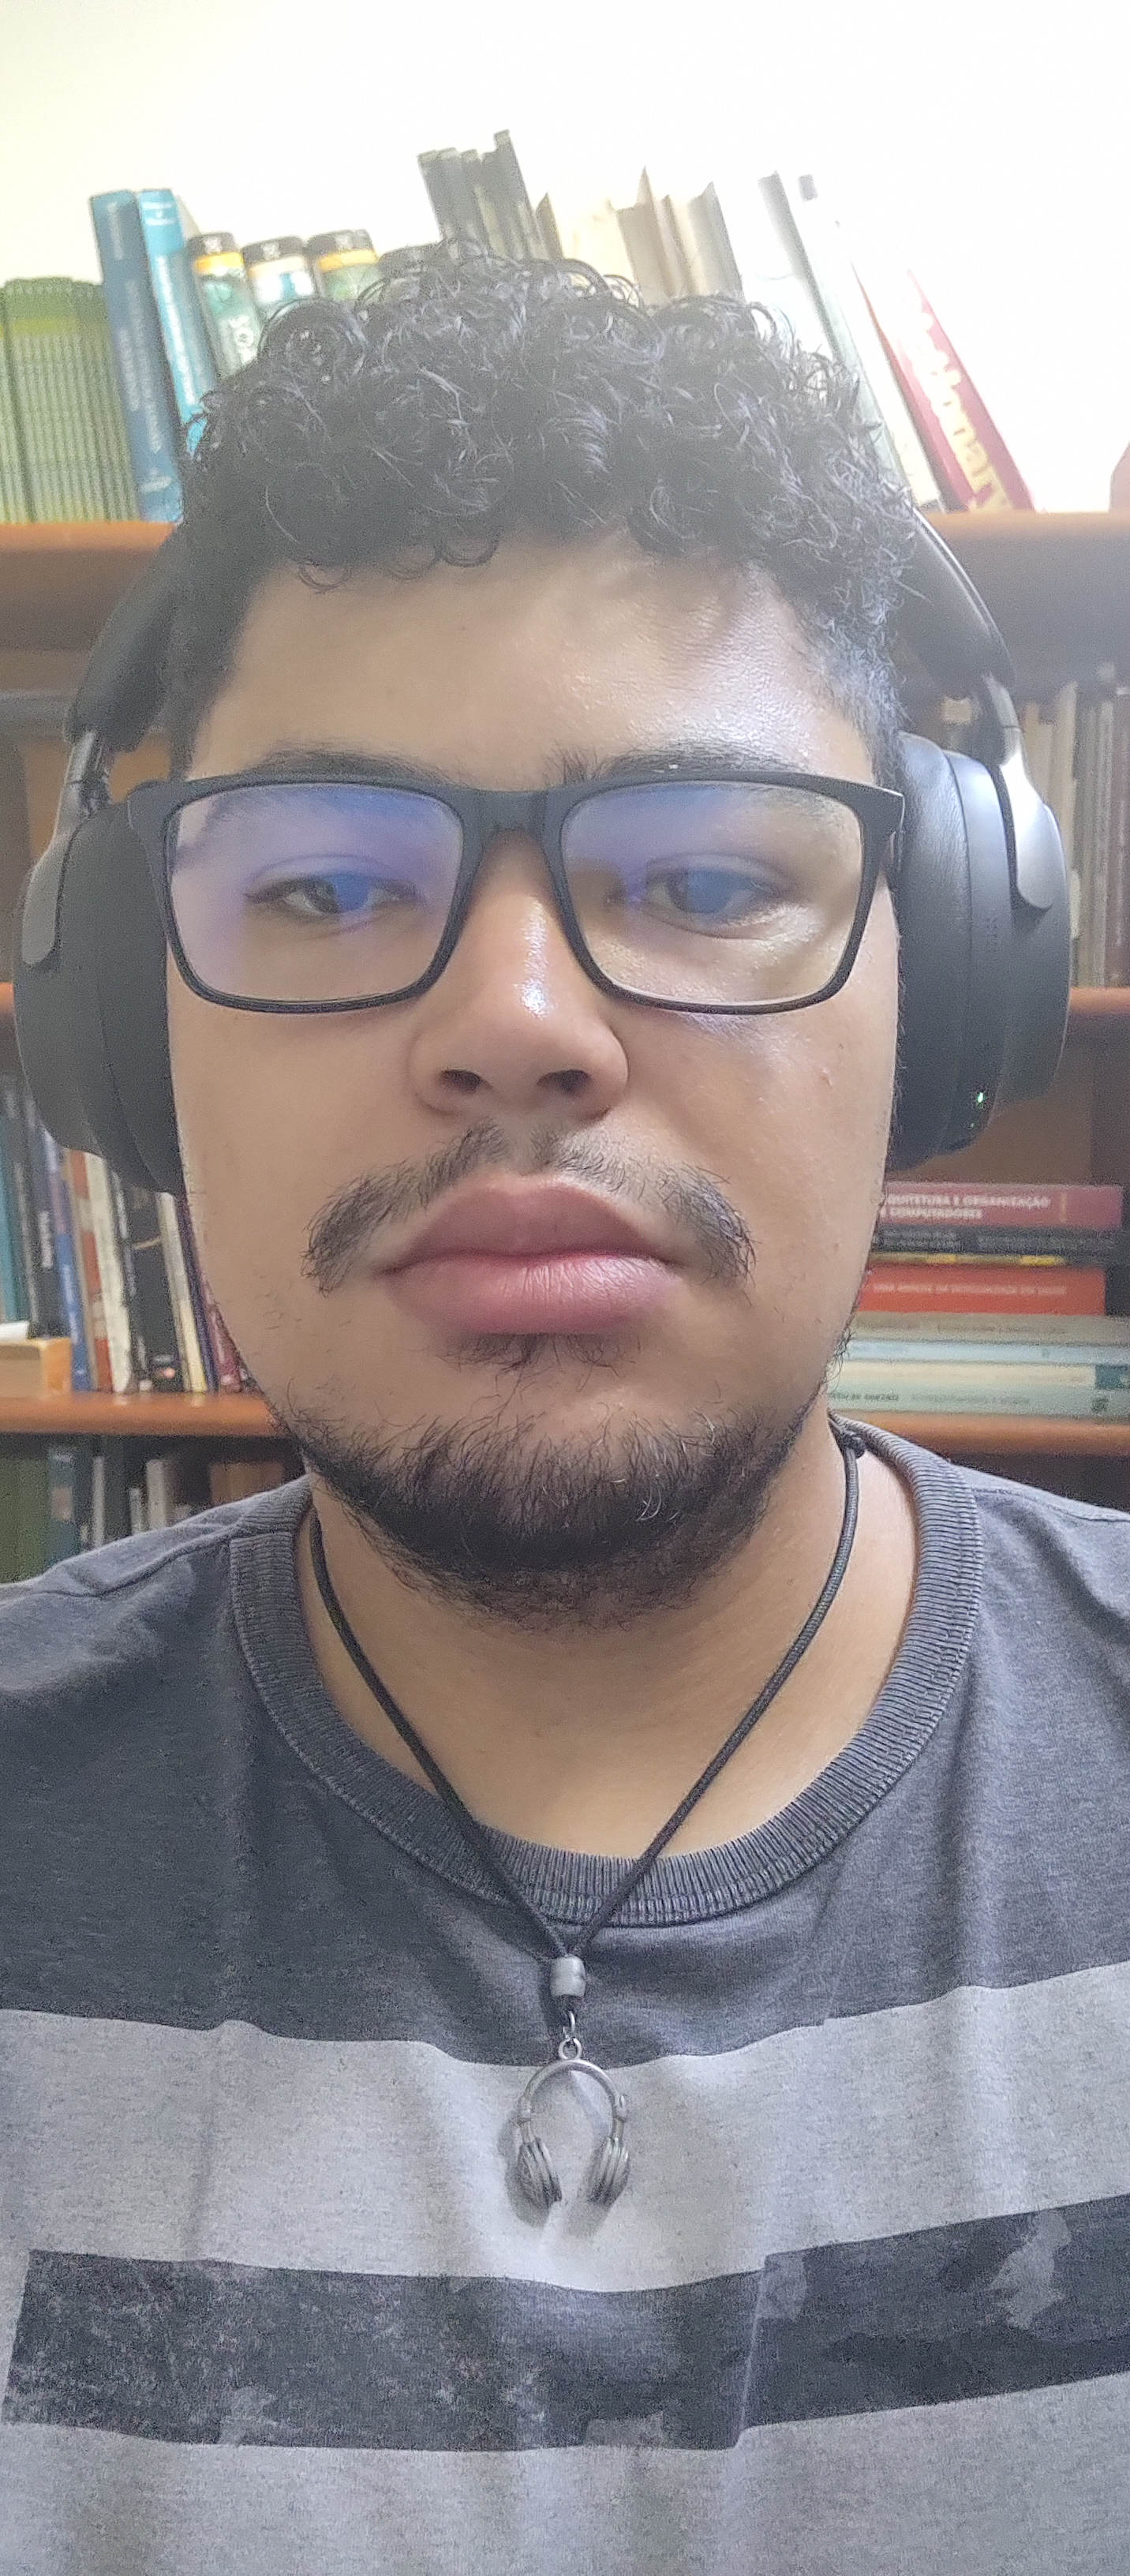
\includegraphics[scale=0.04]{img/downscale_img.png}
        \caption{\label{fig:Rosto_Downscale}Foto com 1/4 do tamanho original.}
    \end{subfigure}
\end{figure}\\
Comparando as imagens \ref{fig:Rosto_grayscale} e \ref{fig:Rosto_Downscale} com a entrada original \ref{fig:Rosto_Full}, não é possível perceber diferença observando as imagens, tanto a saída monocromática quanto
a saída colorida.
Para a obtenção da saída colorida, é necessário fazer a aplicação da redução de tamanho em cada um dos canais \textit{RGB} separados, com a imagem colorida sendo a união dos três após processamento.
O resultado do processamento em cada um dos canais pode ser visto nas imagens resultantes presentes no \href{https://github.com/mutenesss/IPI/tree/trabalho1}{github} do projeto.
\subsubsection{Aumento de Tamanho}
Assim como podemos reduzir o tamanho de uma imagem, podemos também aumentar o tamanho dela, mas agora enfrentamos alguns problemas a mais em comparação ao problema anterior.
Seguindo a ideia anterior de separação do processo em primeiro linhas ou colunas e então aplicar o que não foi anteriormente, fazemos o mesmo para aumento da imagem, primeiro com a criação
de uma matriz com o dobro de linhas e então dobrando o número de colunas utilizando o resultado anterior como base, na forma:
\begin{align}
    \label{math:matrix_double_evens}
    I_{rrows} \in \mathbb{Z}^{2M \times N}, N \in \mathbb{Z}\\
    I_{rcols} \in \mathbb{Z}^{M \times 2N}, M \in \mathbb{Z}\\
    I_{final} \in \mathbb{Z}^{2M \times 2N}, M,N \in \mathbb{Z}
\end{align}\\
Dessa forma, obtemos uma matriz com 4x o tamanho da imagem original, e assim podemos continuar o processo de aumento da imagem. Com o padrão anterior de lidar apenas com índices pares, podemos
preencher os píxeis com índices pares da imagem com os originais, e podemos gerar os píxeis restantes calculando a média dos seus vizinhos, 
onde \[P_{x,y}=\frac{P_{x-1,y} + P_{x+1,y}}{2}\] para as linhas e \[P_{x,y}=\frac{P_{x,y-1} + P_{x,y+1}}{2}\] para as colunas.\\
Um dos problemas que encontramos ao utilizar esse método é o \textbf{overflow}, pois lidamos com $0 \leq P_{x,y}\leq 255$. 
Outros problemas que encontramos são a distorção de cores e também o que fazer quando não temos um vizinho para calcular a média.
\begin{itemize}
    \item \textbf{Overflow:}
    O \textit{OpenCV} utiliza \textit{wraparound} para lidar com o overflow, de forma que valores maiores que o limite levam ao menor valor possível após o limite.
    Uma boa forma de observar isso é no caso $P_{x,y} = 240 + 30$, onde $P_{x,y} = 15$. Esse comportamento pode levar a uma disparidade grande entre a cor ou ao brilho de uma área da imagem, sendo necessário o tratamento para evitar que a mesma ocorra.
    Podemos evitar esse problema de algumas formas, como dividindo ambos os valores de entrada por 2 antes da soma, mas com isso limitamos nosso valor máximo do píxel para 254, 
    além do valor poder estar menor que o calculado pela média por 1 ou 2, algo que se torna um problema ao executar o processo de escala múltiplas vezes.
    Outra forma de lidar com esse problema é usando \textit{typecasting} para permitir que $P_{x,y}$ adote valores maiores que 255, sendo necessário a normalização do valor final e o \textit{typecast} para retornar ao tipo inicial.
    \item \textbf{Ausência de Vizinhos:}
    Ao chegar na linha e na coluna final da imagem, não é possível calcular a média da mesma forma que fizemos para as linhas e colunas anteriores.
    Existem formas de lidar com isso como os métodos de \textit{nearest neighbor} ou \textit{bi-linear interpolation}, mas neste projeto escolhemos a forma mais simples, sendo apenas a cópia da linha e coluna anteriores para preenchimento da imagem. 
\end{itemize}
Utilizando um dos datasets precarregados da biblioteca \textit{scipy}, podemos obter a foto de um guaxinim em meio a grama \ref{fig:guaxinim_full}. 
\begin{figure}[h!t]
    \label{fig:comparação_upscaling}
    \centering
    \begin{subfigure}[ht]{0.5\textwidth}
        \centering
        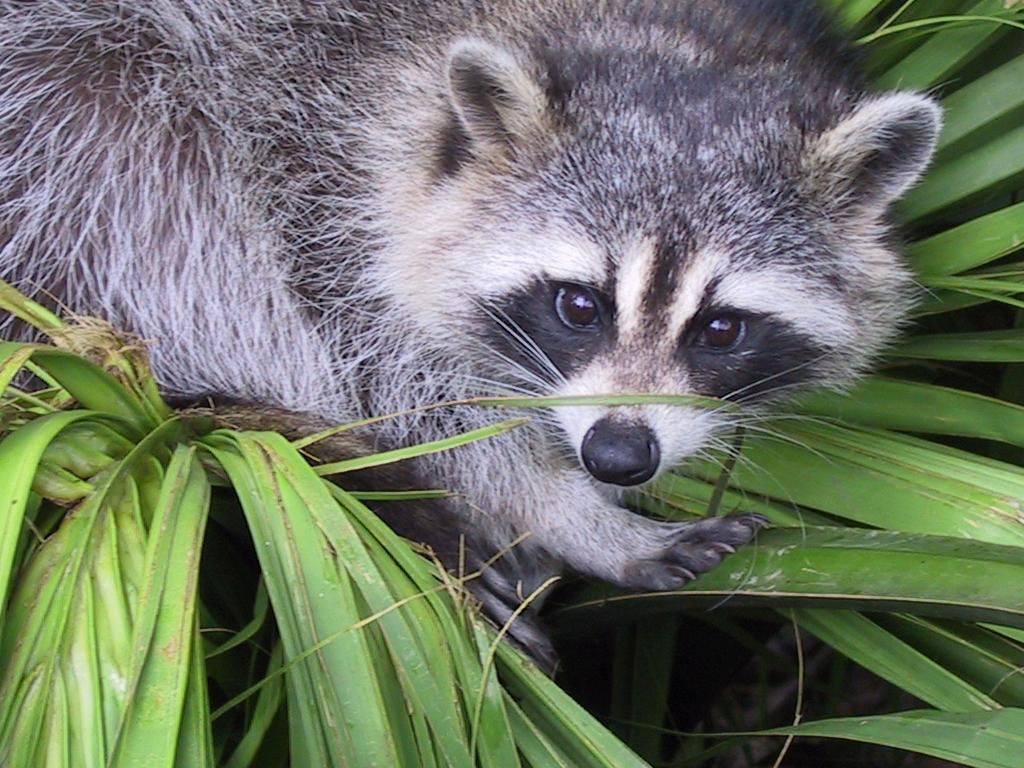
\includegraphics[scale=0.2]{img/face.png}
        \caption{\label{fig:guaxinim_full}Foto original guaxinim.\cite{noauthor_face_nodate}}
    \end{subfigure}
    \quad
    \begin{subfigure}[ht]{0.5\textwidth}
        \centering
        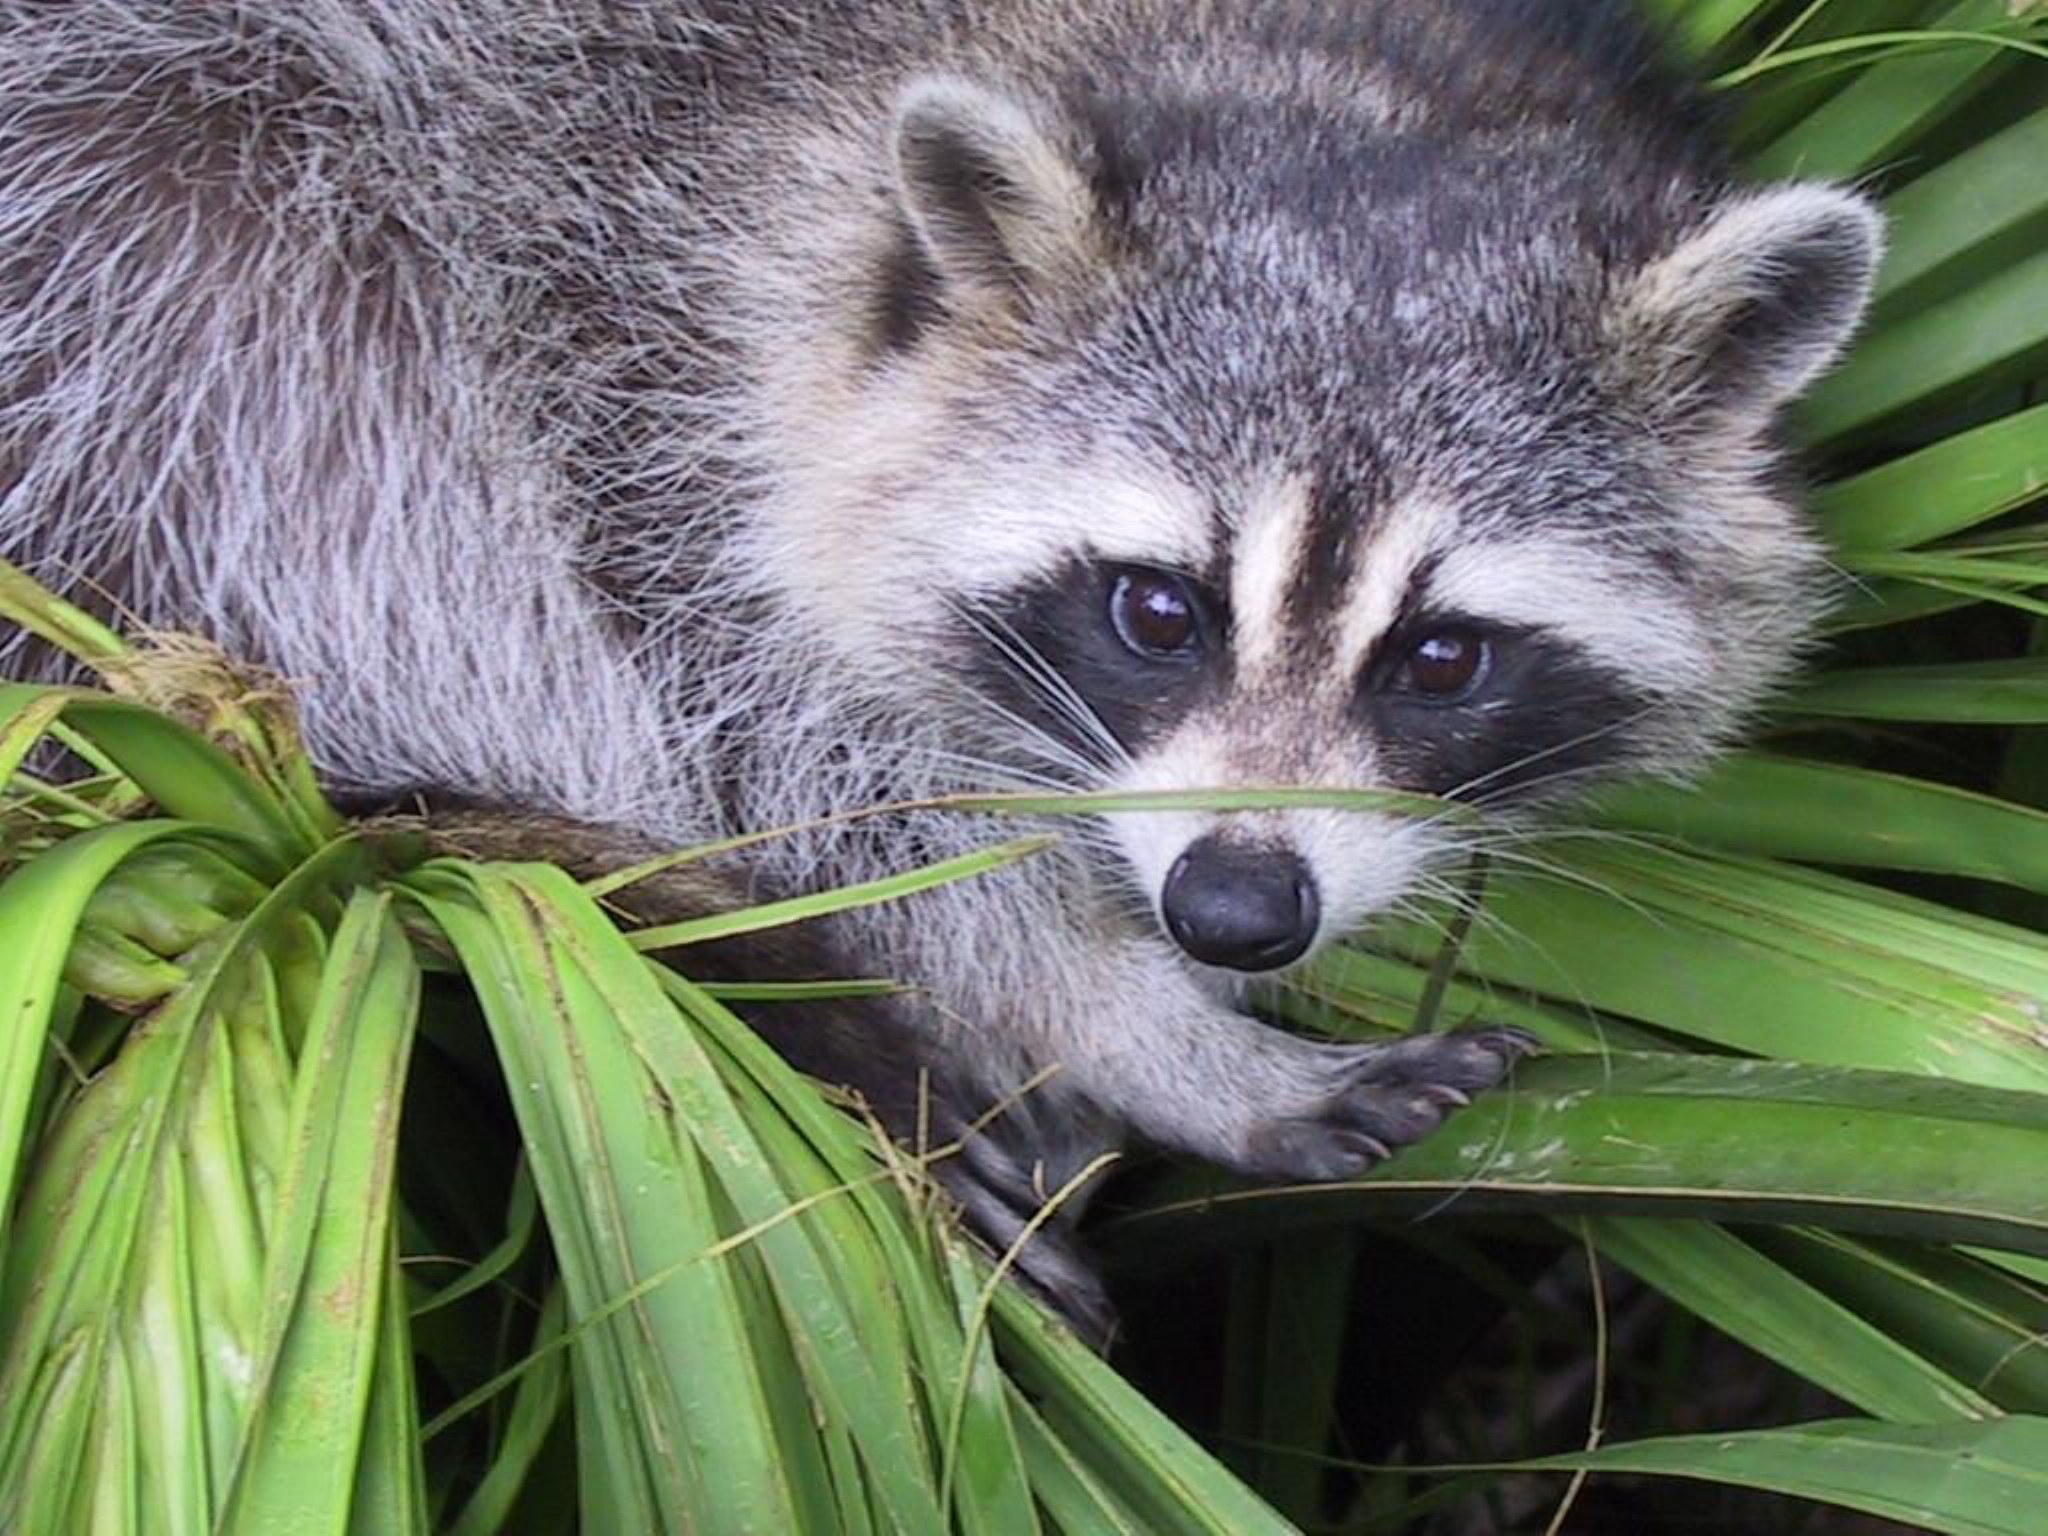
\includegraphics[scale=0.1]{img/upscale_img.png}
        \caption{\label{fig:guaxinim_upscale}Foto do guaxinim após upscaling.}
    \end{subfigure}
\end{figure}\\
Comparando a imagem após o processo de upscaling com a imagem original, é possível visualizar que a imagem com upscale \ref{fig:guaxinim_upscale} fica levemente mais borrada que a imagem original, 
com alguns pontos levemente mais claros e outro mais escuros. 
\subsection{Filtro Laplaciano e Filtro Gaussiano}
Adicionamos agora ao nosso projeto o domínio da frequência. Nesta parte do projeto, é prevista a execução do processo de aguçamento na imagem \textit{Image1.pgm} por uso de filtros Laplaciano e Gaussiano.
\subsubsection[Laplaciano Espacial]{Laplaciano no domínio espacial}
No primeiro ponto exigido dessa parte, é necessária a aplicação de um filtro Laplaciano com kernel de tamanho 3x3, incluíndo diagonais.
Assim, temos um kernel da seguinte forma:
\begin{equation}
    \label{kernel:middle_8}
    k = \begin{pmatrix}
        1 & 1 & 1\\
        1 & -8 & 1\\
        1 & 1 & 1
    \end{pmatrix}
\end{equation}

O resultado da aplicação do filtro laplaciano utilizando o kernel acima pode ser visto na imagem \ref{fig:laplace_border}.\\
Esse resultado obtido deve ser adicionado a imagem original, assim realçando as bordas da imagem original.
\begin{figure}[ht]
    \centering
    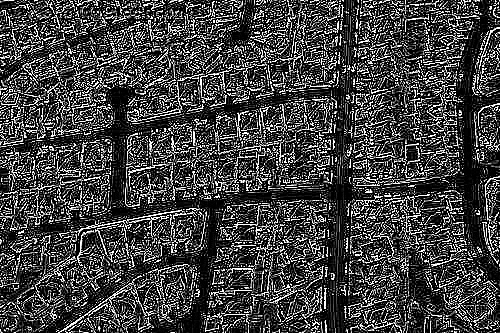
\includegraphics[scale=0.5]{img/ker3_border_aplica_filtro_laplace.png}
    \caption{\label{fig:laplace_border}Bordas obtidas pelo filtro Laplaciano.}
\end{figure}\\
Dentro do \textit{OpenCV} existe uma função chamada \textit{Laplacian}\cite{noauthor_opencv_nodate-1}, que, assim como a implementação manual que nos deu o resultado em \ref{fig:laplace_border}, 
faz a aplicação do filtro Laplaciano para obter as bordas de uma imagem. Ela calcula o operador Laplaciano\cite{noauthor_opencv_nodate} de uma imagem a partir da fórmula
\begin{align}
    \label{math:laplacian_opencv}
    dst=\Delta src=\frac{\delta^2src}{\delta x^2}+\frac{\delta^2src}{\delta y^2}
\end{align}
Dessa forma, o kernel obtido pela função diverge do kernel implementado manualmente,sendo possível perceber as diferenças nas imagens de comparação.
\begin{figure}[ht]
    \centering
    \begin{subfigure}{0.5\textwidth}
        \centering
        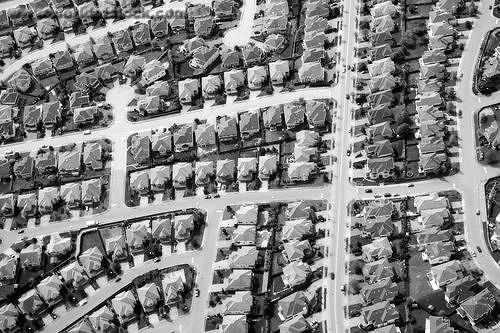
\includegraphics[scale=0.33]{img/image1.png}
        \caption{\label{fig:laplace_original}Imagem inicial para aguçamento das bordas.}
    \end{subfigure}
    \quad
    \begin{subfigure}{0.5\textwidth}
        \centering
        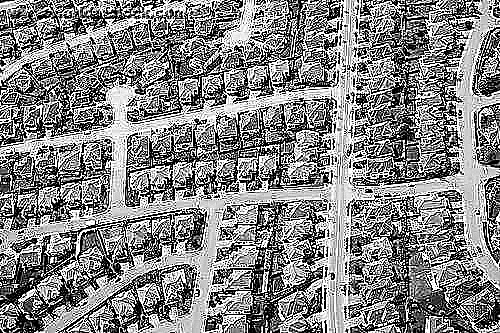
\includegraphics[scale=0.33]{img/ker3_aplica_filtro_laplace.png}
        \caption{\label{fig:laplace_agucado}Imagem após adição das bordas obtidas pelo filtro Laplaciano com kernel manual por meio da função filter2D.}
    \end{subfigure}
    \quad
    \begin{subfigure}{0.5\textwidth}
        \centering
        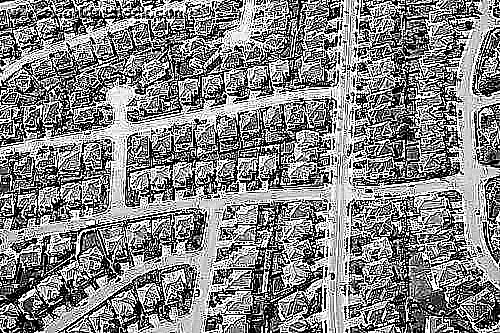
\includegraphics[scale=0.33]{img/lap_aplica_filtro_laplace.png}
        \caption{\label{fig:laplace_agucado_laplacian}Imagem após adição das bordas obtidas pelo filtro Laplaciano por meio da função Laplacian.}
    \end{subfigure}
\end{figure}
\subsubsection[Double filters]{Laplaciano + Gaussiano}
Ainda tratando com imagens no domínio espacial, agora temos a aplicação do filtro Laplaciano e do Blur Gaussiano vindo da função \textit{GaussianBlur}\cite{noauthor_opencv_nodate-1} do \textit{OpenCV}, agora utilizando um kernel
\begin{equation}
    k = \begin{pmatrix}
        0, 1, 0\\
        1,-4, 1\\
        0, 1, 0
    \end{pmatrix}
\end{equation}
e diferentes variâncias($\sigma^2$), podemos comparar o efeito do Blur na imagem, agora desfocando um pouco a imagem.
\begin{figure}[H]
    \centering
    \begin{subfigure}{0.2\textwidth}
        \centering
        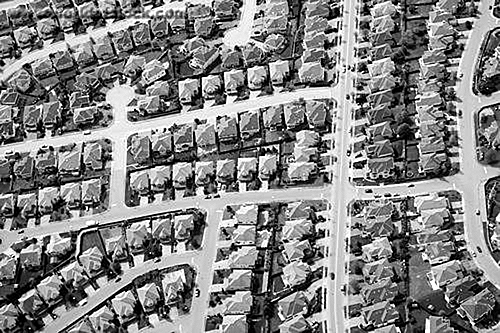
\includegraphics[scale=0.2]{img/0.5_aplica_gaus_laplace.png}
        \caption{\label{fig:var0.5_gauss}Variância = 0.5}
    \end{subfigure}
    \quad
    \begin{subfigure}{0.2\textwidth}
        \centering
        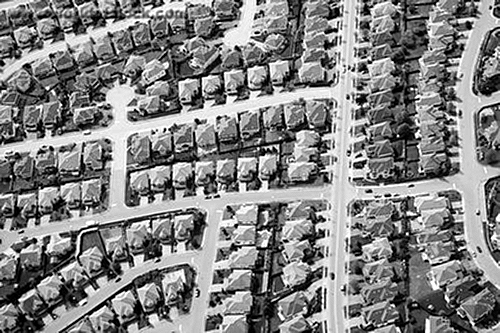
\includegraphics[scale=0.2]{img/1.0_aplica_gaus_laplace.png}
        \caption{\label{fig:var1.0_gauss}Variância = 1}
    \end{subfigure}
\end{figure}

\subsubsection[Ideal_vs]{Ideal vs Gaussiano}
Passando agora para a filtragem no domínio da frequência, iremos fazer a comparação entre um filtro ideal e um filtro Gaussiano, em comparação aos resultados obtidos no domínio espacial.
O filtro ideal escolhido para essa aplicação foi o \textit{High-Pass} ou \textit{Passa-Altas}, com o objetivo de realçar as bordas da imagem, facilitando uma comparação direta com os resultados anteriores.
A fórmula que descreve o filtro ideal passa-baixas para uma dada frequência $D_0$ é
\begin{align}
    H_{low}(k,l) = \begin{cases}
        1, D(k,l) \leq D_0\\
        0, D(k,l) > D_0
    \end{cases}\\
    D(k,l) = \sqrt{(k-\frac{P}{2})^2 + (l-\frac{Q}{2})^2}
\end{align}
Com ($\frac{P}{2},\frac{Q}{2}$) sendo o centro da imagem. O filtro passa-baixas garante que todas as frequências com valor acima de $D_0$ não sejam representadas na imagem.
Esse tipo de filtro é bom para suavizar uma imagem, deixando as bordas menos nítidas. 
Como o filtro que queremos é um que realça bordas, ele é o oposto do passa-baixas, podendo ser calculado como:
\begin{align}
    H_{high}(k,l) = 1 - H_{low}(k,l)
\end{align}
Agora que estamos lidando com o domínio da frequência, a aplicação de um filtro é apenas a passagem de uma função na matriz da imagem, 
em \textit{Python} isso sendo apenas uma multiplicação da matriz de frequência da imagem com a função do filtro.
A obtenção da matriz de frequência de uma imagem ocorre calculando a DFT ou \textit{Discrete Fourier Transform} da imagem e 
aplicando um \textit{shift} para deslocar as frequências periódicas para o centro da imagem. 
Ambas as funções necessárias para essas operações estão presentes na biblioteca \textit{Numpy} do \textit{Python}.
Além do filtro ideal passa-altas, vamos utilizar também um filtro Gaussiano passa-altas, novamente seguindo a fórmula de implementar um filtro passa-baixas e então invertendo o seu valor.
\begin{align}
    H_{low}(k,l) = e^\frac{D^2(k,l)}{2D^2_0}\\
    H_{high}(k,l) = 1 - H_{low}
\end{align}
Para as suas aplicações, definimos os seguintes parâmetros:
\begin{itemize}
    \item $D_0$ do filtro Gaussiano - 80
    \item Frequência de corte do filtro Ideal - 200
\end{itemize}
\begin{figure}[ht]
    \begin{subfigure}{0.5\textwidth}    
        \centering
        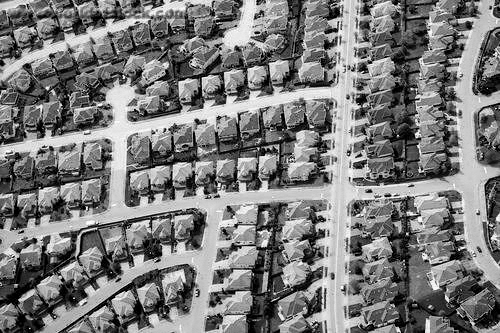
\includegraphics[scale=0.3]{img/compara_ideal_ideal.png}
        \caption{\label{fig:comp_ideal}Aplicação do filtro ideal.}
    \end{subfigure}
    \quad
    \begin{subfigure}{0.5\textwidth}    
        \centering
        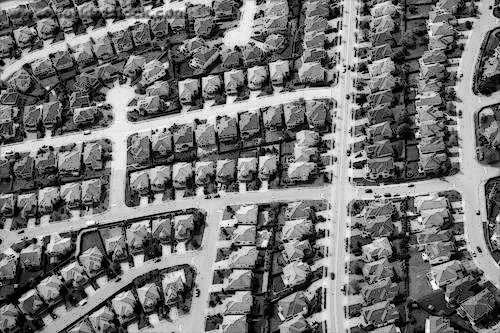
\includegraphics[scale=0.3]{img/compara_ideal_gauss.png}
        \caption{\label{fig:comp_gauss}Aplicação do filtro Gaussiano.}
    \end{subfigure}
\end{figure}

\begin{figure}[H]
    \centering
    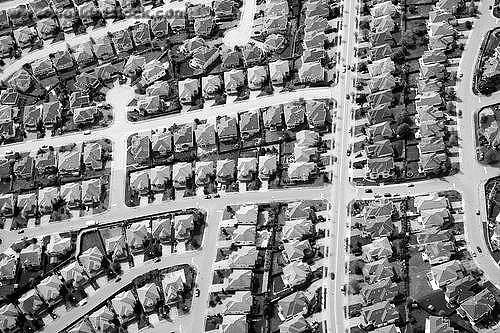
\includegraphics[scale=0.4]{img/compara_ideal_ideal+gaussBlur.png}
    \caption{\label{fig:comp_ideal+gauss}Aplicação do filtro ideal e do Blur Gaussiano no domínio espacial.}
\end{figure}

\section{Conclusões}
Em consideração ao domínio espacial, ao comparar as duas imagens obtidas com o filtro Laplaciano, é possível perceber que a imagem com maior variância \ref{fig:var1.0_gauss} tem suas bordas um pouco menos pronunciadas e é um pouco mais escura que a de menor variância \ref{fig:var0.5_gauss},
sendo a imagem \ref{fig:var1.0_gauss} a melhor das duas, por manter bem os detalhes da imagem inicial sem um brilho muito pronunciado.

Já considerando o domínio da frequência, tanto a imagem obtida utilizando apeans o filtro Gaussiano na frequência \ref{fig:comp_gauss} quanto a imagem obtida utilizando o filtro ideal na frequência e o 
GaussianBlur no domínio espacial \ref{fig:comp_ideal+gauss} podem ser consideradas melhores em relação as imagens obtidas através dos filtros Laplacianos no espaço \ref{fig:laplace_agucado}\ref{fig:laplace_agucado_laplacian}, 
embora ambas mantenham um detalhamento menor das bordas, ainda há um bom nível de detalhamento das mesmas, em conjunto a um nível de claridade geral da imagem mais agradável.

Os resultados obtidos das filtragem, sejam elas sido implementadas manualmente ou utilizando uma função pre-existente das bibliotecas \textit{Numpy} ou \textit{OpenCV} foram satisfatórios,
com a escolha de alguns parâmetros utilizados sendo escolhidos por observação empírica de diversos valores. Algumas das funções implementadas manualmente tem implementação providenciada pela biblioteca \textit{scipy}, 
como o filtro Butterworth, que não foi implementado com sucesso neste trabalho, mas o uso das mesmas no contexto do trabalho levaria apenas a capacidade de leitura da documentação para aplicação da função e não do entendimento de conceitos necessário da matéria. 

\bibliography{IPI}
\end{document}
